\lab{Linsweep Algorithms}{Linsweep Algorithms}{Linesweep Algorithms}

\objective{Learn about and implement a basic linesweep algorithm}

\section*{General Linesweep Algorithms}

Linesweep algorithms are a computationally significant group of algorithms that have a variety of applications. 
In the strictest sense, linesweep algorithms almost always involve use of a priority queue and binary tree to lower the temporal complexity associated with certain tasks. 
Some notable examples include Fortune's Algorithm for calculating voronoi diagrams, and Andrew's Algorithm for computing the convex hull of a set of points. 
Here we will explore a basic linesweep algorithm that allows efficient computation of the smallest distance between any two points in a set of points. 

\section*{Naive Implementation}

The obvious way of doing this is to simply compare each point with each of the other points. 
Since distance is symmetrical, we can compare each point with the points that follow it in the list we are given. 
A good implementation is as follows:

\begin{lstlisting}
def multidist(p0,p1):
    l=len(p0)
    return (sum([(p0[i]-p1[i])**2 for i in range(l)]))**(.5)
def badmindist(X):
    l=len(X)
    r=multidist(X[0],X[1])
    for i in xrange(l):
        for j in xrange(i+1,l):
            d=multidist(X[i],X[j])
            if d<r:
                r=d
    return r
\end{lstlisting}

Since, on average, we iterate through half the list per point added, this algorithm will have complexity $O(n^2)$. 
You may verify this numerically. 
For very small numbers of points, it may be faster to use this function, but this algorithm quickly becomes inefficient for all but the smallest numbers of points. 
This leads us to next option. 
A linesweep algorithm.

\section*{A Simplified Linesweep Algorithm}

A more efficient way of doing this exact same thing is to order the points in the list, then iterate through them and only consider the points that are within a given range about the point you are processing. 
In this case, this is what makes this a line sweep algorithm. 

Instead of ordering the points in a list, it is more efficient to order them in a priority queue. 
We have implemented a very basic priority queue in the file \li{pqueue.py}. 
A more complex priority queue can be found in the library \li{Queue} that is included in Python. 
For this lab, we have implemented a simpler version for you. 
The simpler queue we have implemented is faster but less general. 
The points can be added into the queue by using the \li{add(data,priority)} method for the priority queue object. 
You can get the next item in the priority queue using the \li{get()} method. 
In this case you will want to add points into the queue with priority equal to their $x$-value. 
If their $x$-values are equal, they will be returned in the order they are entered. 
You could give a tuple for the order of the point, then the queue would order them by $x$ value and then, when $x$ values are equal, by $y$ value, but that is more expensive computationally and it makes no difference in the actual implementation of the algorithm. 

For small data sets, we can simply make a list of "active" points which have $x$ values greater than that of the point we are currently processing, but less than the smallest distance we have encountered thus far. 
As we iterate through the points, we can remove the points that are no longer relevant to callculation and only interate over the ones we are concerened about. 
This, again is much like a queue. 
To implement this algoritm we recommend you use the \li{deque} object from the \li{collections} library. 
This will give a sleight speed up over lists for large data sets. 

We first process the first two points, add them to our active queue and set the minimum distance to be the distance between them. 
We then pull out the next point in our priority queue. 
Using the point we just pulled out, we remove any points we can from the active list, then we compare the distance between the active points and the point we are processing. 
If the distance from any of our active points is less than the smallest distance we have already recorded, we set the minimum to be the new smallest distance. 
When we have done this for all of the points in the set, we will have passed the points where the minimum distance occurs and our function can return the actual minimum distance for any two points within the set.

This algorithm can be illustrated as follows:

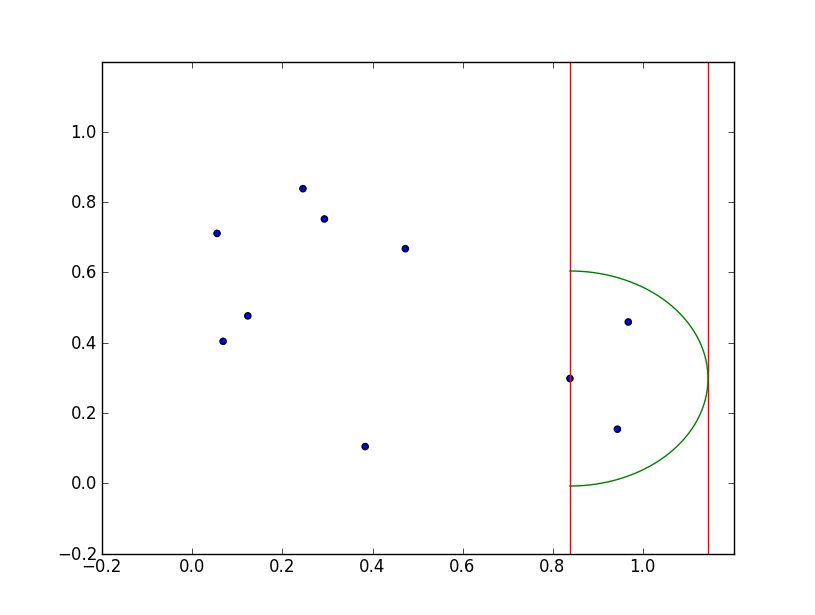
\includegraphics[width = \textwidth]{simple1.png}
After processing the first two points, we process the third point and see that our minimum distance thus far has dropped.

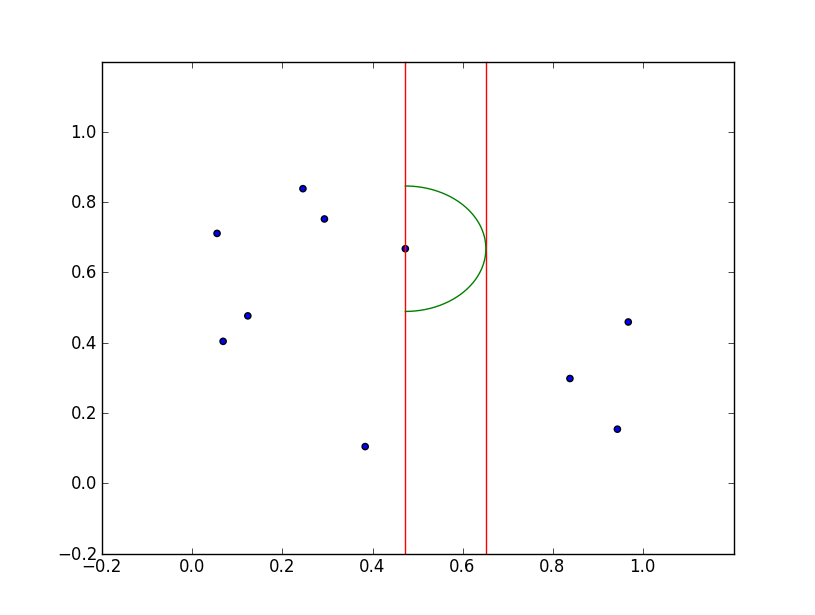
\includegraphics[width = \textwidth]{simple2.png}
This change in the minimum thus far is reflected in how we form the actives list for the next point we process. 
We remove the points from the top of the queue that are too far away in the $x$ direction to have a distance less than the current minimum. 
We then process anything that is left.

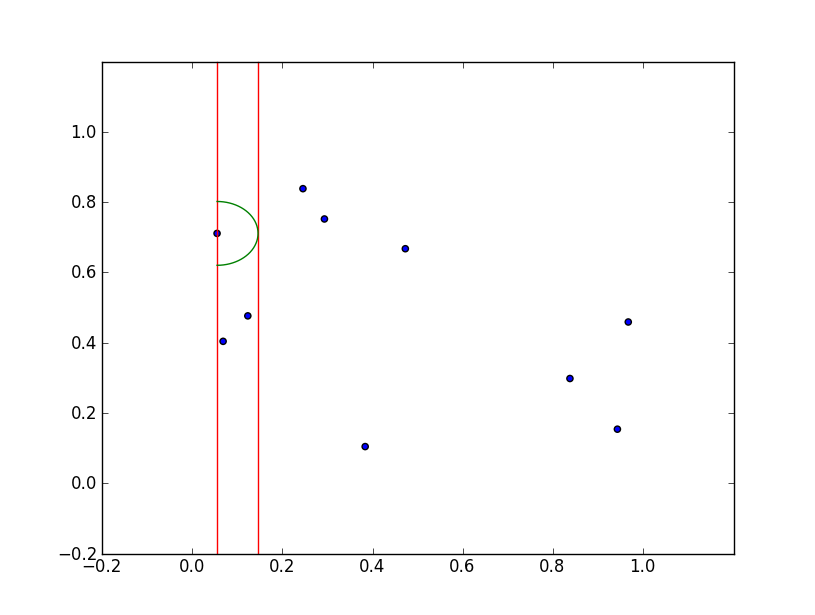
\includegraphics[width = \textwidth]{simple8.png}
After iterating over all the points in the set, we have the final minimum distance desired.

\begin{problem}
Implement the above linesweep algorithm using python.
\end{problem}

\section*{A Linesweep Algorithm}

You may have noticed that we are not exploiting all of the symmetry of the problem in the previous algorithm. 
It would likely speed things up if we could also slice away the points that have $y$ values that could not possibly yield the minimum distance. 
The list operations involved in doing this are somewhat more involved. 
In order to slice the list effectively, we will need to order our active points with respect to their $y$ values, but continue to remove them according to their $x$ value. 
There are a variety of ways this can be done. 
Many linesweep algorithms would use a binary tree to store these points and get good insertion and deletion times. 
This is doable, but in this case, except for very poorly conditioned problems, our actives list tends to remain small, so we can do this with a list. 

To speed up this algorithm, we will need to flip the order of the values in the points, then store them in the actives list in order. 
Flipping the coordinates in the actives list allows us to use the default ordering of tuples that is built in to python. 
To do this insertion, we will use a binary search over the list. 
The functions \li{bisect_left} and \li{bisect_right} from the \li{bisect} module will do this for you. 
A binary search over a list works under the assumption that the list is already ordered and gives you a fast way to know where to insert an item in your ordered list. 
At each iteration, we will first remove the points that no longer are important to the points we are processing. 
We will then iterate only over the pertinent part of the actives list, according to the range of $y$ values that are close to the point we are processing.

For speed, when updating the active list, you should modify the list in place. 
What this means is that instead of removing each point individually as you iterate over the list, you should do something like \li{actives[:] = [p for p in actives if (p[1] - x) <= r]} 
Using a list comprehension in this way allows you to filter out the points you need to remove without so many repeated list operations. 

A good way to iterate over a sublist of a list is to use an iterator object. 
The function \li{islice} for the \li{itertools} library will let you do what you need. 
You should use a binary search to figure out where you need to cut your list. 

Also, for large numbers of points, you will want to import the functions you call into the local namespace to save on lookup time. 
For each function, you can do this using a line of code that is something like \li{islice = it.islice}. 

This algorithm can be illustrated as follows:


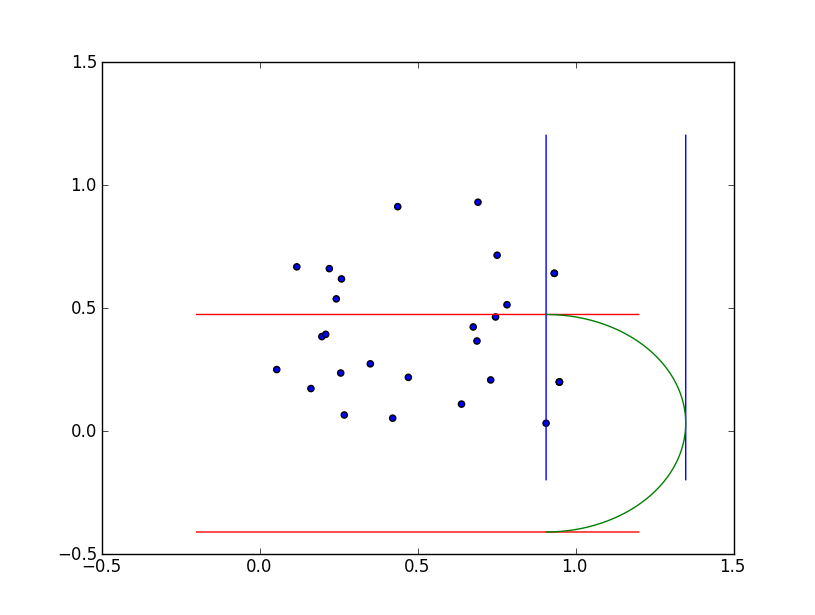
\includegraphics[width = \textwidth]{ptsweep1.png}
In processing the first point, we find find that we must reduce the radius. Notice that we only need to consider the points that lie in the box formed by the red an blue lines.


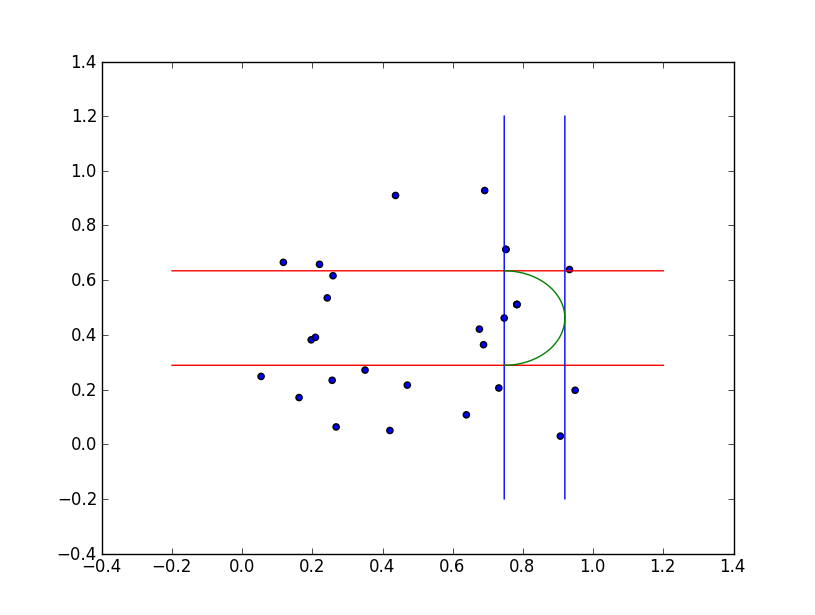
\includegraphics[width = \textwidth]{ptsweep4.png}
A few more points along, we find that we mus reduce our minimum radius significantly.

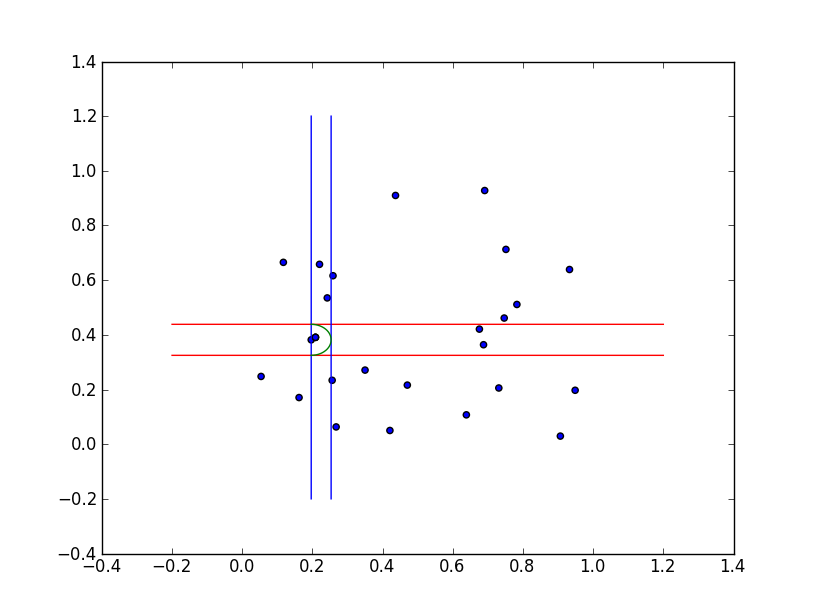
\includegraphics[width = \textwidth]{ptsweep20.png}
This is where we actually hit the minimum distance.

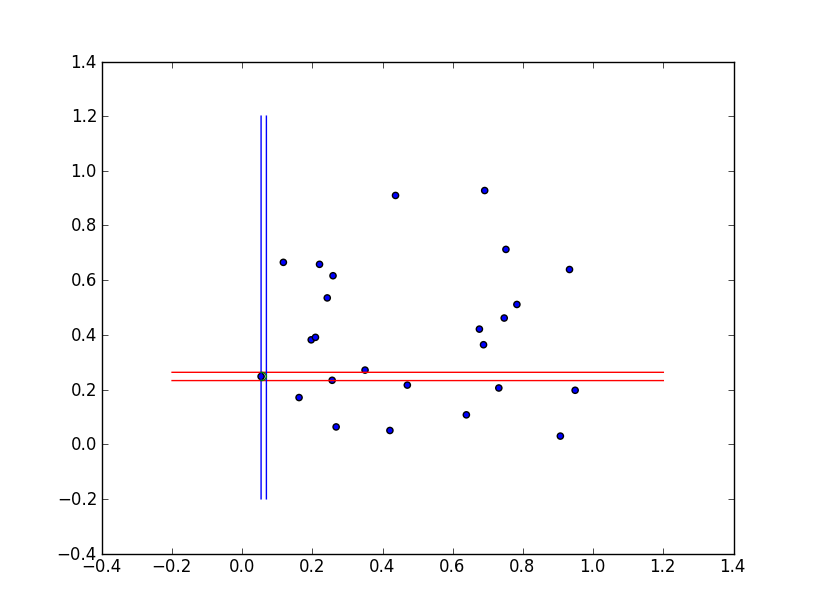
\includegraphics[width = \textwidth]{ptsweep23.png}
After processing through all the points, we are guaranteed to have hit the minimum distance already, so our minimum distance thus far is our final return value.

\begin{problem}
Implement the algorithm above. 
Time it against the naive implementation at the beginning of this lab and against the simplified version you coded above.
\end{problem}

\begin{problem}
Modify your code so that it returns the coordinates of the two points that are closest together in addition to the distance between them.
\end{problem}

\begin{problem}
Modify the functions you have so that they can process points in higher dimensions. 
Try processing randomly generated higher dimensional data sets. 
What do you observe about the complexity of the problem as the number of dimensions increases?
\end{problem}

Depending on the symmetry of the problem, you can implement different versions of this algorithm. 
In higher dimensions, you can slice the actives list along differend axes, but this may not actually yield a speed increase. 
This is because, again, due to the conditioning of the problem, the size of the active list does not usually warrant the extra operations involved. 

There are a variety of ways this algorithm can be implemented, and the actual performance for a real world problem will depend on your ability to exploit the symmetry of the situation at hand. For most situations, the version using lists will probably be the fastest. 
